% Walls or cascade? -- the confined-MHD paper.
%
% Build: make (in this directory), or latexmk -pdf main.tex.
% Every number below that comes from a run is printed by numbers.py, which also
% writes the four tab_*.tex files; the figures are made by
% tools/plot_tg_mhd_ladder.py (see the Makefile). Formatted for Physics of
% Plasmas with REVTeX 4.2; the text is journal-neutral.
\documentclass[aip,pop,reprint,amsmath,amssymb,superscriptaddress,floatfix]{revtex4-2}

\usepackage[utf8]{inputenc}
\usepackage[T1]{fontenc}
\usepackage{graphicx}
\usepackage{bm}
\usepackage[hidelinks]{hyperref}
\graphicspath{{../../results/P_tg_mhd/fig/}}

\newcommand{\Rey}{\mathrm{Re}}
\newcommand{\vv}{\bm{v}}
\newcommand{\BB}{\bm{B}}
\newcommand{\eps}{\varepsilon}

\begin{document}

\title{Walls or cascade? A pre-registered test of wall dissipation in decaying
magnetohydrodynamic turbulence}

\author{Alessandro De Rosis}
\email{alessandro.derosis@manchester.ac.uk}
\affiliation{The University of Manchester, Manchester M13 9PL, United Kingdom}
% TODO(author): department line.

\date{\today}

\begin{abstract}
Does the small-scale dissipation of magnetohydrodynamic (MHD) turbulence come from
the cascade in the bulk, as in a periodic box, or from the walls that confine
laboratory plasmas and liquid metals? We test this with a controlled numerical
experiment. The symmetries of the Taylor--Green MHD flow make the box $[0,\pi]^3$ a
closed domain with free-slip, perfectly conducting walls: solving that box directly
reproduces the periodic flow to round-off, and making its walls no-slip, with
everything else unchanged, isolates what the walls do. With two independent lattice
Boltzmann implementations we follow the decay at unit magnetic Prandtl number for
Reynolds numbers $250$ to $2000$, on grids that resolve the $\Rey^{-1/2}$ wall layer,
with the observable, the resolution criterion and the decision rule fixed before the
runs. No-slip walls add dissipation within $\Rey^{-1/2}$ of them at every Reynolds
number and under every definition we tried. The excess is viscous: the near-wall
Ohmic dissipation is 40--45\% lower than with free-slip walls. Snapshots and
three-dimensional views of the local dissipation show current sheets crossing the
near-wall layer of the free-slip box and a broad viscous layer at the no-slip walls. The pre-registered
reading, the excess at the dissipation peak, falls from $0.063$ to $0.036$ between
$\Rey=1000$ and $2000$, the outcome we had called ``cascade''. That fall is set by
which of two maxima of the dissipation is the larger: the peak switches between
rungs, and over a factor of eight in Reynolds number the trend of the wall share
depends on when it is measured, while its sign does not.
\end{abstract}

\maketitle

%===============================================================================
\section{Introduction}
%===============================================================================

Decaying magnetohydrodynamic (MHD) turbulence has been studied mostly in periodic
boxes.\cite{mininni2006,lee2008,pouquet2010,mininni2009,linkmann2015} There the
dissipation is made in current and vorticity sheets that the cascade forms in the
bulk, and its rate tends to a value independent of the Reynolds number,
$\Rey$,\cite{mininni2006,mininni2009,linkmann2015} the MHD counterpart of the finite
dissipation of hydrodynamic turbulence.\cite{sreenivasan1998}

The flows that motivate much of this work, in liquid metals and laboratory plasmas,
are bounded, and walls add boundary layers that dissipate. Whether that dissipation
survives as the viscosity vanishes is a question about the walls themselves. Kato
showed that a Navier--Stokes flow in a bounded domain converges to its Euler limit if
and only if the dissipation in a layer of thickness proportional to the viscosity
vanishes.\cite{kato1984} In two-dimensional hydrodynamics, Nguyen van yen, Farge and
Schneider found dissipating structures produced at no-slip walls whose dissipation
appears to tend to a finite value as $\Rey$ grows.\cite{nguyen2011} Confined MHD
turbulence has been simulated with volume penalisation in two\cite{neffaa2008} and
three\cite{morales2014} dimensions. We are not aware of a comparison that changes only
the wall condition and follows the answer as $\Rey$ increases.

We therefore ask: in decaying three-dimensional MHD turbulence, does a no-slip wall
take a share of the dissipation that holds as $\Rey$ grows (``walls''), or does that
share fall, so that the periodic picture of a bulk cascade survives confinement
(``cascade'')?

The answer rests on a construction that isolates the walls. The Taylor--Green (TG)
MHD flows of Lee \textit{et al.}\cite{lee2008} and Pouquet
\textit{et al.},\cite{pouquet2010} which generalize the hydrodynamic TG
vortex,\cite{brachet1983} are symmetric about the faces of $[0,\pi]^3$. On
those faces the velocity is impermeable and free-slipping, and the magnetic field has
the parity of a perfect conductor or, for a second field, of a pseudo-vacuum. The
periodic flow restricted to $[0,\pi]^3$ is therefore exactly the flow in a closed box
with those walls. We solve that box directly, with walls on lattice nodes, and check
that it reproduces the periodic flow to round-off. We then change the velocity
condition from free slip to no slip and nothing else. The difference between the two
boxes is the effect of the walls.

A question with two outcomes invites an analysis flexible enough to find either. We
therefore fixed the observable, the resolution criterion and the decision rule in
version-controlled job scripts before the runs they
govern,\cite{nosek2018,gelman2014} and we report them as fixed.
Section~\ref{sec:method} describes the problem, the method and the protocol,
Sec.~\ref{sec:verify} the verification, Sec.~\ref{sec:results} the results, and
Sec.~\ref{sec:discussion} what they settle and what they do not. In brief, the
no-slip excess is robust: it is positive at every $\Rey$ and under every definition
we tried, it is viscous, and it comes with less near-wall Ohmic dissipation than free
slip. The pre-registered verdict is ``cascade''. But that verdict rests on a switch
between two maxima of the dissipation, and over the factor of eight in $\Rey$ that one
GPU affords, the trend of the wall share depends on when it is measured.

%===============================================================================
\section{Problem, method and protocol}
\label{sec:method}
%===============================================================================

\subsection{The flow and the box}

We solve the incompressible visco-resistive MHD equations in units where the initial
velocity amplitude and the density are one,
\begin{align}
  \partial_t \vv + (\vv\cdot\nabla)\vv &= -\nabla p + (\nabla\times\BB)\times\BB
     + \nu\nabla^2\vv, \label{eq:ns}\\
  \partial_t \BB &= \nabla\times(\vv\times\BB) + \eta\nabla^2\BB, \label{eq:ind}
\end{align}
with $\nabla\cdot\vv=\nabla\cdot\BB=0$ and $\nu=\eta=1/\Rey$, so the magnetic Prandtl
number is one and $\Rey=1000$ is run C2 of Ref.~\onlinecite{pouquet2010}. Lengths are
in units of $1/k_0$, where $k_0=1$ is the wavenumber of the TG velocity below, so the
box has side $\pi$; velocities are in units of its initial amplitude $v_0$; times are in
units of $1/(k_0v_0)$, about one large-eddy turnover time; and the magnetic field is in
Alfv\'en units, $\BB/\sqrt{\mu_0\rho}$, which is why Eq.~(\ref{eq:ns}) carries no
$\mu_0$. Every quantity is therefore dimensionless: $\Rey=v_0/(k_0\nu)$, energies are
per unit mass, and dissipation rates are in units of $k_0v_0^3$. Most of what follows
needs no units at all, being shares of the total dissipation or densities relative to
the box mean. The initial conditions are those of
Refs.~\onlinecite{lee2008,pouquet2010}:
\begin{align}
  \vv &= (\sin x\cos y\cos z,\; -\cos x\sin y\cos z,\; 0), \label{eq:v0}\\
  \BB_C &= b_0\,(\sin 2x\cos 2y\cos 2z,\; \cos 2x\sin 2y\cos 2z, \nonumber\\
        &\qquad\quad -2\cos 2x\cos 2y\sin 2z), \label{eq:bc}\\
  \BB_I &= b_0\,(\cos x\sin y\sin z,\; \sin x\cos y\sin z, \nonumber\\
        &\qquad\quad -2\sin x\sin y\cos z), \label{eq:bi}
\end{align}
with $b_0=1/\sqrt3$, so that the kinetic and magnetic energies,
$E_V=\langle|\vv|^2\rangle/2$ and $E_M=\langle|\BB|^2\rangle/2$, are both $1/8$ at
$t=0$.

On the six faces of $[0,\pi]^3$ the velocity~(\ref{eq:v0}) has $\vv\cdot\bm{n}=0$ and
$\partial_n\vv_t=0$: an impermeable, free-slip wall. The field $\BB_C$ has
$\BB\cdot\bm{n}=0$ and $\partial_n\BB_t=0$. This is what a perfectly conducting wall
imposes, since $\bm{n}\times\bm{E}=0$ with Ohm's law
$\bm{E}=\eta\bm{j}-\vv\times\BB$ and $\vv\cdot\bm{n}=\BB\cdot\bm{n}=0$ gives
$\bm{n}\times\bm{j}=0$, and it holds with either velocity condition. The field $\BB_I$
has $\BB\times\bm{n}=0$ and $\partial_n B_n=0$, the pseudo-vacuum condition. These
parities are preserved by Eqs.~(\ref{eq:ns})--(\ref{eq:ind}). The boxes are:
\begin{description}
\item[A] free slip, conducting walls, $\BB_C$: an exact restriction of the periodic
flow, and the control;
\item[B] no slip, conducting walls, $\BB_C$: the experiment, which differs from A in
the velocity condition only;
\item[C] no slip, no field: the hydrodynamic reference;
\item[A$'$, B$'$] as A and B, with $\BB_I$ and pseudo-vacuum walls.
\end{description}
The TG velocity does not vanish on the faces, so a no-slip box starts impulsively: its
wall nodes are set at rest at $t=0$, and a vortex sheet on every wall dominates the
early dissipation. In B the dissipation rate at $t=0$ is $\eps=0.30$, $0.22$, $0.15$
and $0.09$ at $\Rey=250$, $500$, $1000$ and $2000$, $95$--$98$\% of it within
$\Rey^{-1/2}$ of the walls.

\subsection{Lattice Boltzmann discretization}

The velocity is carried by a D3Q27 distribution with a central-moment collision in a
shifted basis,\cite{geier2006,derosis2018} and the Maxwell stress enters its
equilibrium.\cite{dellar2002} The field is carried by Dellar's vector-valued
distribution\cite{dellar2002} on D3Q7 with a single-relaxation-time collision; $\nu$
and $\eta$ set the two relaxation times.\cite{kruger2017} The box has $N$ nodes a side
with the walls on nodes $0$ and $N-1$, so the spacing is $h=\pi/(N-1)$. The lattice
velocity of the unit velocity is $u_0=0.05$, one step is $\Delta t=u_0h$, and
$\nu_{\mathrm{lat}}=u_0/(h\Rey)$; the fluid relaxation parameter is
$\tau-\tfrac12=3\nu_{\mathrm{lat}}$, and the magnetic one is $4\eta_{\mathrm{lat}}$
on D3Q7. Table~\ref{tab:runs} lists the runs.

\begin{table}
\caption{\label{tab:runs}Runs: two grids per rung. $\delta/h$ is the number of
lattice spacings in the layer thickness $\delta=\Rey^{-1/2}$; $\tau-\frac12$ is the
fluid relaxation parameter; steps to $t=10$ and the largest lattice Mach number over A
and B are for the finer grid; ``bits'' is the floating-point precision.}
\begin{ruledtabular}
\begin{tabular}{rcccccc}
$\mathrm{Re}$ & $N$ & $\delta/h$ & $\tau-\tfrac12$ & steps & $\mathrm{Ma}_{\max}$ & bits \\
\hline
125 & 128, 192 & 3.62, 5.44 & 0.0485, 0.0730 & 12159 & 0.094 & 64 \\
250 & 192, 256 & 3.85, 5.13 & 0.0365, 0.0487 & 16234 & 0.102 & 64 \\
500 & 256, 384 & 3.63, 5.45 & 0.0244, 0.0366 & 24383 & 0.109 & 64 \\
1000 & 384, 512 & 3.86, 5.14 & 0.0183, 0.0244 & 32531 & 0.117 & 64 \\
2000 & 512, 640 & 3.64, 4.55 & 0.0122, 0.0153 & 40680 & 0.133 & 32 \\
\end{tabular}

\end{ruledtabular}
\end{table}

All walls are on nodes, and each wall node collides like any other once its unknown
populations are set. For free slip these are the mirror images of their partners
about the wall (specular reflection). For no slip we use the regularized velocity
condition of Latt \textit{et al.}\cite{latt2008} with zero wall velocity; at the
twelve edges and eight corners, where it has no density stencil, the density is set
to one. For the field we use a parity wall. Write the field component $a$ as carried
by its own populations $g^{(a)}_i$. At a node on a wall normal to axis $k$, every
population $i$ entering the box is replaced by
\begin{equation}
  g^{(a)}_i \leftarrow s_{ak}\, g^{(a)}_{i^*},
  \label{eq:parity}
\end{equation}
where $i^*$ is the mirror of $i$ about the wall and $s_{ak}=-1$ if the wall flips
component $a$ (the normal one, $a=k$, at a conducting wall; the tangential ones,
$a\ne k$, at a pseudo-vacuum wall) and $+1$ otherwise. At edges and corners the mirrors
compose and the signs multiply. A conducting wall thus flips only the normal
component, and a pseudo-vacuum wall only the tangential ones. Dellar has given
moment-based magnetic boundary conditions for the same
distribution;\cite{dellar2013} Eq.~(\ref{eq:parity}) is a population-level mirror
that imposes a parity on any combination of faces. Three tests in the repository
check it. First, with free slip and either parity, the box of $N$ nodes reproduces
the periodic $2\pi$ box of $2(N-1)$ nodes to $10^{-14}$, node for node and transient
included. Second, $\BB\cdot\bm{n}$ on the wall nodes stays at $10^{-32}$. Third, in
the no-slip box the exact decay of the conducting-wall eigenmode
$\BB=B_0(\sin x\cos y,-\cos x\sin y,0)$, which leaves the fluid at rest, converges at
second order (order $2.00$ over $N=17$, $33$, $65$).

The method exists in two implementations that share no source code: one in C++20 on
Kokkos,\cite{edwards2014,trott2022} one in CUDA. Their host builds agree to every
printed digit over 815 steps at $N=65$, $\Rey=200$, with free and no slip. The CUDA
build on the device agrees with the Kokkos reference to within $6\times10^{-16}$ of
each diagnostic's scale. The production runs used NVIDIA A100 (80\,GB) GPUs: double
precision up to $\Rey=1000$, and single precision at $\Rey=2000$, where $N=640$ fits
in memory only in single precision. The runs reported here took 34 GPU-hours.

\subsection{Diagnostics}

The dissipation rate is $\eps=\nu\langle|\bm{\omega}|^2\rangle+\eta\langle|\bm{j}|^2\rangle$,
with $\bm\omega=\nabla\times\vv$ and $\bm{j}=\nabla\times\BB$. The box average
$\langle\cdot\rangle$ uses trapezoidal weights, $\tfrac12$ on a face, $\tfrac14$ on an
edge and $\tfrac18$ at a corner, which makes the box average of a mirror-symmetric
field equal to its periodic average exactly. Derivatives are second-order central
differences, extended at a wall by the wall's own rule: the mirror for a free-slip
velocity and for the magnetic parity, and a one-sided second-order stencil for a
no-slip velocity.

Each node is at distance $d=kh$ from its nearest wall, $k=0,1,\dots$ With the
trapezoidal weights, the nodes with $d=kh$ fill exactly the part of the box at
distances between $(k-\tfrac12)h$ and $(k+\tfrac12)h$ from the walls (between $0$ and
$h/2$ for the wall nodes). If $e_k$ is the dissipation in layer $k$, the dissipation
within a distance $rh$ of the walls is
\begin{equation}
  \mathcal{E}(r) = \sum_{j<k} e_j + \bigl(r-k+\tfrac12\bigr)\, e_k,
  \qquad k=\lfloor r+\tfrac12\rfloor,
  \label{eq:within}
\end{equation}
that is, linear within each layer (with $\mathcal{E}=2re_0$ for $r<\tfrac12$). The
share of the dissipation within $m\delta$ of the walls, $\delta=\Rey^{-1/2}$, is
\begin{equation}
  f_m(t) = \mathcal{E}(m\delta/h) \Big/ \textstyle\sum_k e_k, \qquad m=1,2,4,
  \label{eq:fw}
\end{equation}
and it divides into a viscous and an Ohmic part, $f_m=f_m^{\nu}+f_m^{\eta}$, each a
share of the total $\eps$. The dissipation density relative to the box mean is a
layer's share of $\eps$ over its share of the volume.

Counting whole node layers instead (every node with $kh<m\delta$) measures a layer of
thickness $(\lceil m\delta/h\rceil-\tfrac12)h$ rather than $m\delta$: $0.91\delta$ at
$N=384$ and $1.07\delta$ at $N=512$ for $\Rey=1000$. In our first set of ladder runs
this made $f_1$ differ by 8--25\% between the two grids of a rung while $\eps$ agreed
to 1\%. Swept across $N=33$ to $49$ at fixed physics, the count makes $f_4$ jump
between $0.52$ and $0.60$ each time $4\delta/h$ crosses a node, while
Eq.~(\ref{eq:within}) keeps it within $0.561$--$0.566$. Any layer, shell or threshold
observable on a lattice can do this.

We also use, after the fact (Sec.~\ref{sec:windows}), the time-integrated share over
a window $[t_0,t_1]$,
\begin{equation}
  F_m = \int_{t_0}^{t_1} f_m\,\eps\,dt \Big/ \int_{t_0}^{t_1}\eps\,dt ,
  \label{eq:F}
\end{equation}
the fraction of all the energy dissipated in the window that was dissipated within
$m\delta$ of the walls. It is evaluated with the trapezoidal rule over the probes,
which are $0.05$ or $0.1$ apart, with every integrand interpolated to the window's
edges.

\subsection{The pre-registered protocol}
\label{sec:protocol}

The two outcomes of Sec.~I were stated, qualitatively, on 25 September 2026, before any
production run. The following rules were committed with the job scripts before the runs
they govern.
The observable and the gate were committed with the ladder on 27 September 2026. The
estimator of $f_m$ was corrected on 28 September, after the first ladder failed the
gate for the reason given above; the observable it estimates and the gate did not
change. The Mach control was fixed on 29 September, and the rule for the top rung on
30 September. Both came after the lower rungs had been run and before the runs they
judge.
\begin{enumerate}
\item \emph{Observable}: B$-$A in $f_1$ at each run's turbulent dissipation peak. The
peak is the maximum of $\eps$ after $\eps$ has first risen 5\% above its running
minimum, refined by a parabola through the three probes around the discrete maximum;
$f_m$ is interpolated to that time. The rule skips the impulsive start of a no-slip
box; for free slip the peak is the global maximum. A run in which $\eps$ never rises
5\% above its running minimum has no turbulent peak and no $f_m$.
\item \emph{Resolution gate}: at every (box, $\Rey$), $f_1$, $f_2$ and $f_4$ at the
peak agree within 5\% (relative) between the two grids.
\item \emph{Band}: the grid differences of $f_1$ for A and for B, added.
\item \emph{Decision}: ``walls hold'' if B$-$A at the top rung lies within the combined
bands of its value at the rung below; otherwise ``cascade''.
\item \emph{Controls}, each changing one thing: $u_0$ halved at $\Rey=500$ and $1000$,
which halves the Mach number and $\tau-\frac12$ together; and double against single
precision at $\Rey=2000$, $N=512$. A control passes if it moves B$-$A by less than the
band.
\end{enumerate}
The time-integrated share~(\ref{eq:F}) was not part of the protocol; we introduce it
in Sec.~\ref{sec:windows} because of what Sec.~\ref{sec:switch} found.

%===============================================================================
\section{Verification}
\label{sec:verify}
%===============================================================================

The free-slip box A at $\Rey=1000$ is run C2 of Pouquet \textit{et
al.}\cite{pouquet2010} Its minimum ratio of magnetic to kinetic energy is
$E_M/E_V=0.3695$ and $0.3693$ at $N=384$ and $512$, reached at $t=7.3$, against
their $0.35$. The first maximum of $\Omega_M/\Omega_V$ after its initial fall is
$2.154$ and $2.159$, against their ``2.''. Here $\Omega_V$ and $\Omega_M$ are the
kinetic and magnetic enstrophies. Our ratio is converged to four figures between the
two grids and lies $5.5$\% above theirs, which is quoted to two figures. A run at
$N=97$ gave $0.357$, closer to their value but at $t=9.8$ on an under-resolved grid.

Table~\ref{tab:verify} shows the resolution gate. Every rung of A and B with a
turbulent peak passes it, the worst difference being $3.0$\% in $f_1$ of A at
$\Rey=2000$. Without a turbulent peak by $t=10$ on either grid are B at $\Rey=125$ and
C at $\Rey\le500$; C at $\Rey=2000$ is still rising at $t=10$. Halving $u_0$ moves B$-$A
by $-0.0014$ at $\Rey=500$ and by $-2\times10^{-5}$ at $\Rey=1000$, against bands of
$0.0030$ and $0.0004$. Double precision at $\Rey=2000$ moves it by less than
$10^{-5}$ against $0.0021$, although the two runs differ by up to $4\times10^{-5}$
(relative) in their time series. All three controls pass. Over every run, the total
mass drifts by at most $4.4\times10^{-5}$ (relative), and the r.m.s.\ of $\nabla\cdot\BB$ stays below $1$\% of the r.m.s.\ of
$|\bm{j}|$. The largest lattice Mach number is $0.133$, in A at $\Rey=2000$
(Table~\ref{tab:runs}).

\begin{table*}
\caption{\label{tab:verify}Resolution gate and controls. Relative differences of
$f_1$, $f_2$ and $f_4$ at the turbulent peak between the two grids of each rung, the
band of B$-$A (the two grid differences of $f_1$, added), and the shift of B$-$A in
the control run: Mach, $u_0$ halved; FP64, double precision at $N=512$.}
\begin{ruledtabular}
\begin{tabular}{rccccl}
$\mathrm{Re}$ & $N$ & A: $\Delta f_1/\Delta f_2/\Delta f_4$ (\%) & B: $\Delta f_1/\Delta f_2/\Delta f_4$ (\%) & band & control shift \\
\hline
250 & 192, 256 & 0.7/0.2/0.1 & 1.0/0.7/0.2 & 0.0020 & -- \\
500 & 256, 384 & 0.8/0.5/1.0 & 2.1/1.5/0.7 & 0.0030 & Mach, $-0.0014$ \\
1000 & 384, 512 & 0.7/0.7/0.3 & 0.2/0.1/0.2 & 0.0004 & Mach, $<10^{-4}$ \\
2000 & 512, 640 & 3.0/1.3/0.8 & 0.5/0.4/0.3 & 0.0021 & FP64, $<10^{-4}$ \\
\end{tabular}

\end{ruledtabular}
\end{table*}

%===============================================================================
\section{Results}
\label{sec:results}
%===============================================================================

\subsection{Where the dissipation sits}
\label{sec:where}

Figure~\ref{fig:ladder}(a) shows how the dissipation is spread across the box at
$\Rey=1000$, integrated over $t=2$--$10$. At the walls, the dissipation density is
$8.50$ times the box mean in C, $2.43$ times in B and $0.38$ times in A. The
free-slip conducting walls are quieter than the bulk. The no-slip walls of the MHD
box are more active than the bulk, but much less so than those of the hydrodynamic
box. In C the density falls below the mean beyond $d\approx4\delta$: in that box the
walls do most of the dissipating. Over $t=2$--$10$, C dissipates $33$\% of its energy
within $\delta$ of the walls and B $9.9$\%. At its own turbulent peak ($t=3.20$), C's
$f_1$ is $0.50$. C carries half of B's initial energy, since it has no field. This is
the one rung at which both boxes have a turbulent peak, so it is the one rung at which
they can be compared.

\begin{figure*}
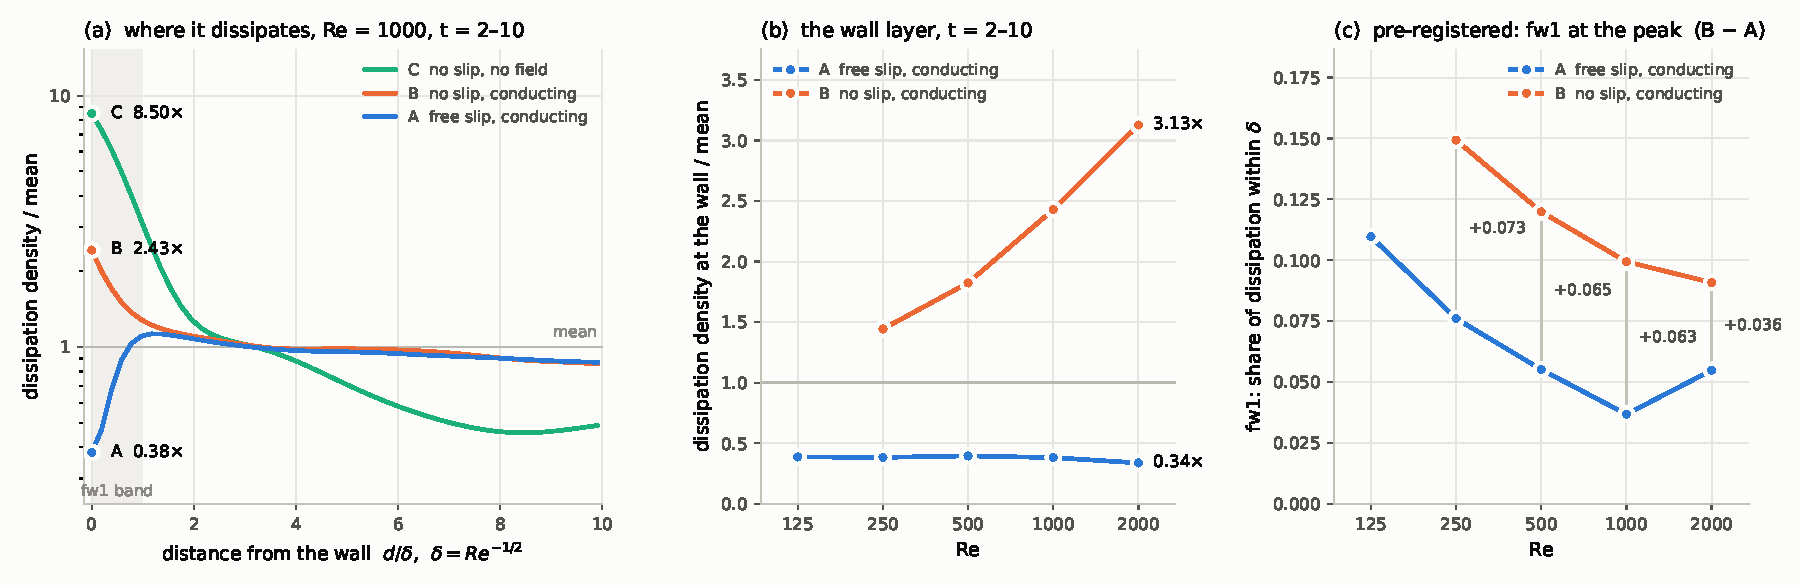
\includegraphics[width=\textwidth]{tg_mhd_ladder.pdf}
\caption{\label{fig:ladder}Where the dissipation sits. (a) Dissipation density
relative to the box mean against distance from the walls, $d/\delta$ with
$\delta=\Rey^{-1/2}$, at $\Rey=1000$, integrated over $t=2$--$10$; the shaded layer is
that of $f_1$. (b) The density at the walls against $\Rey$, over the same window.
(c) The pre-registered observable: $f_1$ at each run's turbulent dissipation peak,
with B$-$A at each rung. Each point is from the finer grid of its rung (Table~\ref{tab:verify}).}
\end{figure*}

Figure~\ref{fig:ladder}(b) follows the density at the walls with $\Rey$. In B it rises
monotonically, $1.44$, $1.82$, $2.43$ and $3.13$ times the mean at
$\Rey=250$--$2000$. In A it stays near $0.38$ and falls to $0.34$ at $\Rey=2000$. B's
wall density rises monotonically in each of the five time windows of
Sec.~\ref{sec:windows}, as $\Rey^{0.25}$ to $\Rey^{0.44}$ depending on the window. A's
changes as $\Rey^{-0.02}$ to $\Rey^{-0.11}$.

\subsection{The no-slip excess and what it is made of}
\label{sec:excess}

Table~\ref{tab:results} and Fig.~\ref{fig:windows}(b) give the time-integrated share
$F_1$ over $t=2$--$10$. No-slip walls take more of the dissipation next to them at
every rung: B$-$A $=0.059$, $0.055$, $0.054$ and $0.048$ at $\Rey=250$--$2000$, with
grid bands of at most $0.0009$. The excess is viscous. Its viscous part is $+0.072$
to $+0.059$ and its Ohmic part is \emph{negative}, $-0.014$ to $-0.011$. That deficit
is not an artefact of dividing by a larger total. Over the window the no-slip box
dissipates \emph{less} energy than the free-slip one ($0.55$--$0.72$ of the initial
energy, against $0.62$--$0.75$), so its near-wall Ohmic dissipation is lower in
absolute terms too, $0.55$--$0.59$ of A's. In A the Ohmic part is the larger of the
two near the walls: $0.039$ against $0.030$ at $\Rey=250$, and $0.026$ against $0.012$
at $\Rey=2000$.

\begin{table*}
\caption{\label{tab:results}Results on the finer grid of each rung. At the peak:
$t_p$, the time of the turbulent dissipation peak in units of $1/(k_0v_0)$, and B$-$A
in $f_1$ there, the
pre-registered observable. Integrated: the share $F_1$ of the dissipation over
$t=2$--$10$ within $\delta$ of the walls, and the viscous and Ohmic parts of B$-$A.
The grid bands of the integrated B$-$A are at most $0.0009$.}
\begin{ruledtabular}
\begin{tabular}{rcccccccc}
 & \multicolumn{3}{c}{at the peak (pre-registered)} & \multicolumn{5}{c}{integrated, $t=2$--$10$} \\
\cline{2-4}\cline{5-9}
$\mathrm{Re}$ & $t_p^{\mathrm{A}}$ & $t_p^{\mathrm{B}}$ & B$-$A & $F^{\mathrm{A}}$ & $F^{\mathrm{B}}$ & B$-$A & viscous & Ohmic \\
\hline
250 & 2.01 & 1.90 & $+0.073$ & 0.069 & 0.128 & $+0.059$ & $+0.072$ & $-0.014$ \\
500 & 2.23 & 2.14 & $+0.065$ & 0.056 & 0.111 & $+0.055$ & $+0.069$ & $-0.014$ \\
1000 & 4.06 & 2.34 & $+0.063$ & 0.046 & 0.099 & $+0.054$ & $+0.065$ & $-0.012$ \\
2000 & 4.45 & 4.53 & $+0.036$ & 0.038 & 0.086 & $+0.048$ & $+0.059$ & $-0.011$ \\
\end{tabular}

\end{ruledtabular}
\end{table*}

\begin{figure*}
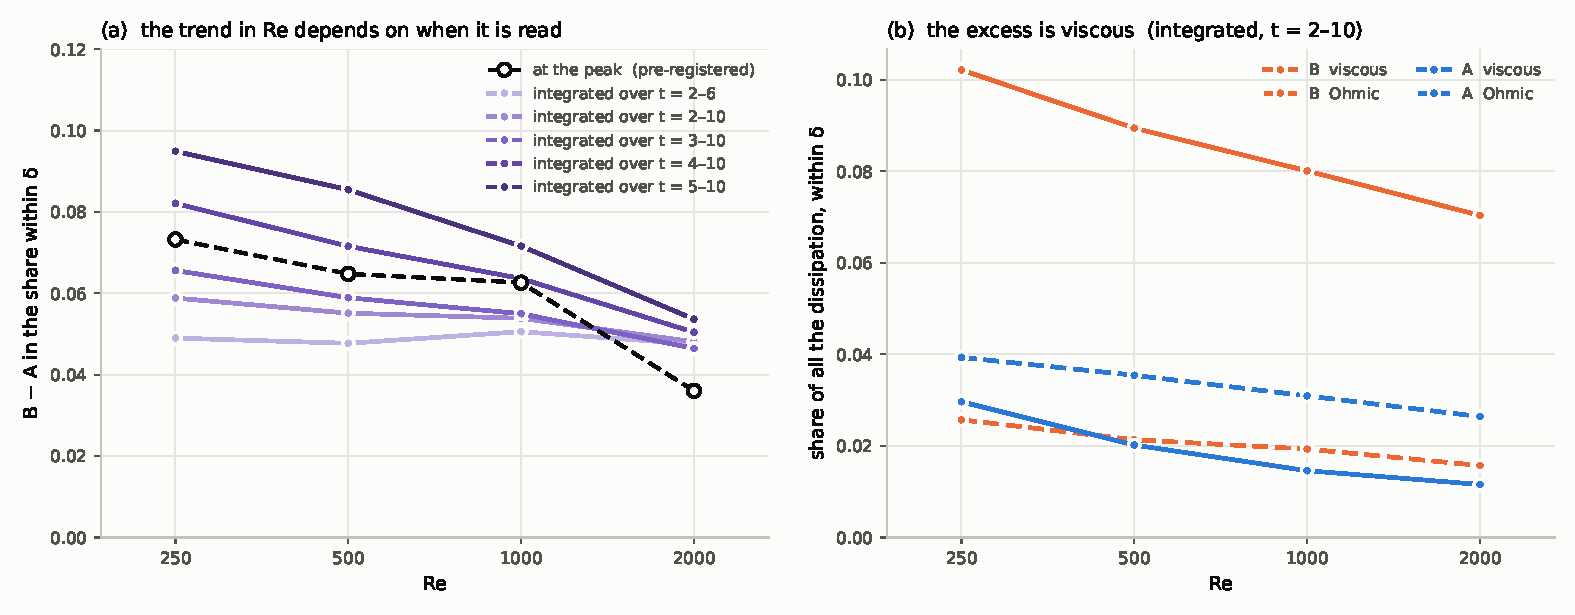
\includegraphics[width=\textwidth]{tg_mhd_windows.pdf}
\caption{\label{fig:windows}(a) B$-$A in the share of the dissipation within $\delta$
of the walls against $\Rey$: at the turbulent peak, as pre-registered (dashed), and
integrated over five time windows, after the fact (light to dark: later windows).
(b) The integrated share $F_1$ over $t=2$--$10$ for A and B, divided into its viscous
and Ohmic parts. Grid bands are at most $0.001$, smaller than the symbols.}
\end{figure*}

\subsection{The pre-registered verdict}
\label{sec:verdict}

Read at the turbulent peak, as registered, B$-$A is $0.0732$, $0.0648$, $0.0626$ and
$0.0361$ at $\Rey=250$--$2000$ [Fig.~\ref{fig:ladder}(c)], with bands of $0.0020$,
$0.0030$, $0.0004$ and $0.0021$. From $\Rey=1000$ to $2000$ it falls by $0.0266$,
$10.5$ times the two rungs' bands added. By the rule fixed before the $\Rey=2000$
runs, the outcome is ``cascade''.

\subsection{The peak switches}
\label{sec:switch}

\begin{figure*}
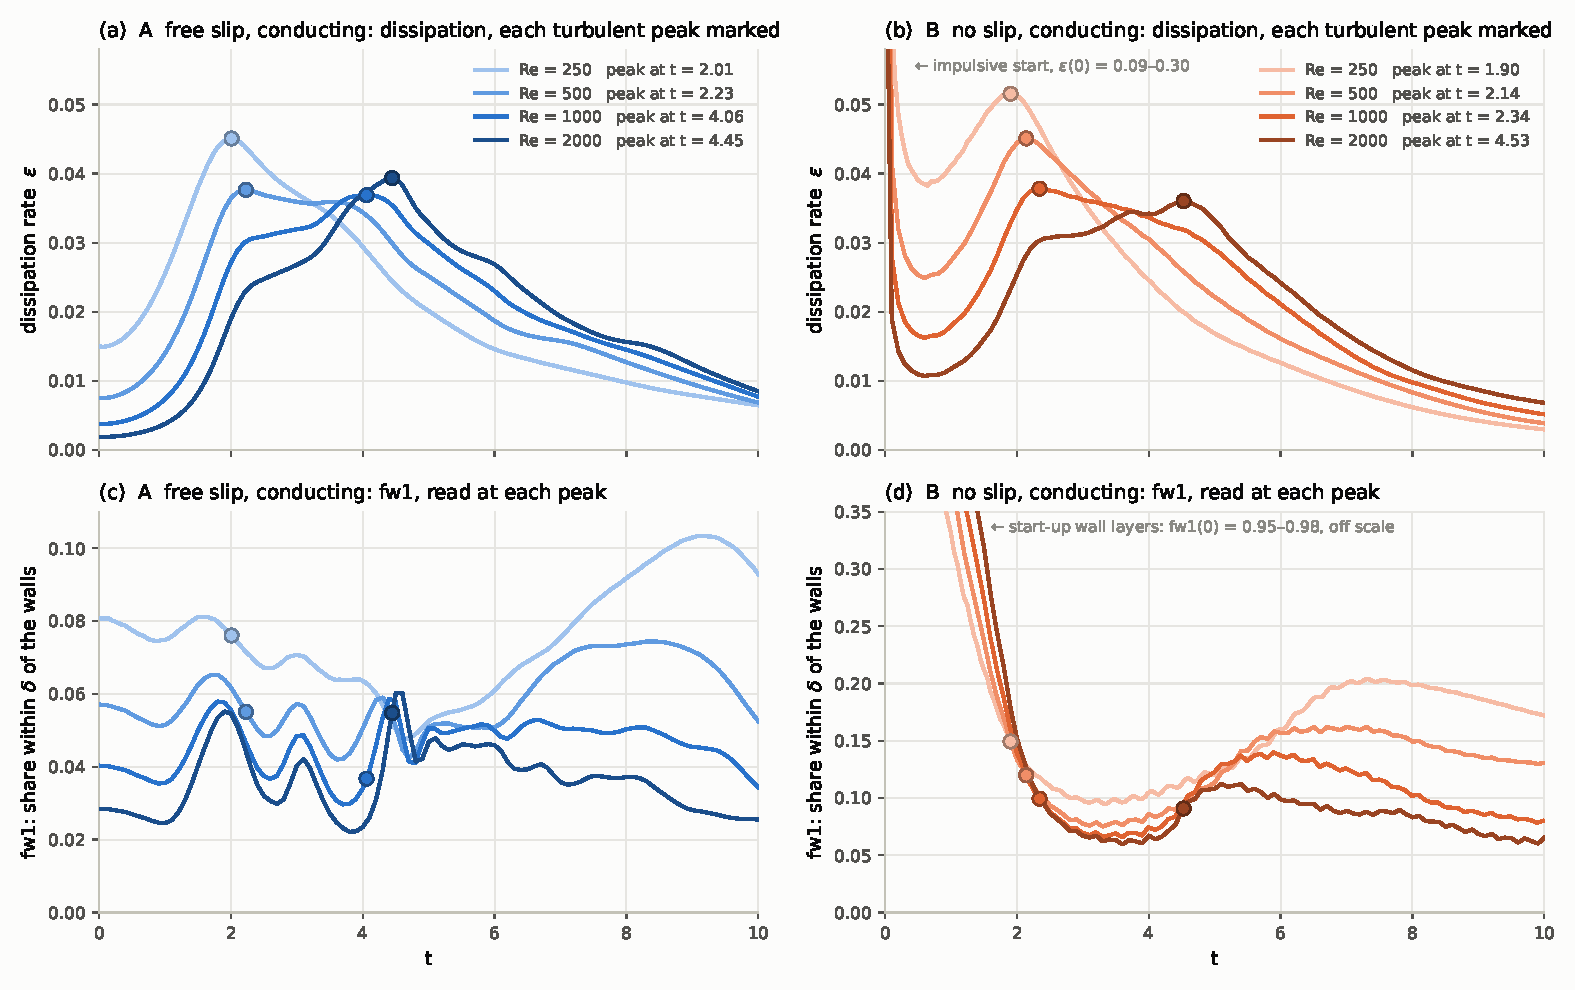
\includegraphics[width=\textwidth]{tg_mhd_peaks.pdf}
\caption{\label{fig:peaks}The turbulent peak switches. The dissipation rate $\eps(t)$,
in units of $k_0v_0^3$ (a, b), and the share within $\delta$ of the walls, $f_1(t)$
(c, d), for the free-slip
box A (a, c) and the no-slip box B (b, d) at $\Rey=250$--$2000$ (light to dark). Dots
mark each run's turbulent peak and the $f_1$ read there. A's early maximum is the
larger up to $\Rey=500$ and its later one from $\Rey=1000$; B's switches between
$\Rey=1000$ and $2000$. B starts off scale at $t=0$ (impulsive start). Time is in
units of $1/(k_0v_0)$.}
\end{figure*}

Figure~\ref{fig:peaks} shows why the last step is not what it seems. The dissipation
of A has an early maximum near $t=2.2$ and a later one at $t=3.6$--$4.4$. At
$\Rey=500$ they are $5$\% apart; from $\Rey=1000$ the later one is the larger, and
A's peak time jumps from $2.23$ to $4.06$. B's peak moves the same way between
$\Rey=1000$ and $2000$, from $2.34$ to $4.53$: at $\Rey=2000$ its early rise is only a
shoulder [Fig.~\ref{fig:peaks}(b)].

And $f_1$ does not vary slowly through either maximum. A's oscillates with a period
near $1.3$, between $0.022$ and $0.060$ at $\Rey=2000$. B's falls from $0.32$ at
$t=1.5$ to $0.06$ at $t=3.7$ as the start-up layers decay, then rises to about $0.11$
[Fig.~\ref{fig:peaks}(c, d)]. The pre-registered reading therefore compares the two
boxes at different times: at $\Rey=1000$, B at $t=2.34$ and A at $t=4.06$. Between
$\Rey=1000$ and $2000$ it moved from a time at which B$-$A, compared at equal times, is
near $0.06$ at both Reynolds numbers ($0.059$ and $0.064$ at $t=2.3$) to one at which it
is near $0.03$ at both ($0.035$ and $0.028$ at $t=4.5$). At equal times, B$-$A does
not fall with $\Rey$ up to $t\approx4$: at $t=3.5$ it is $0.034$--$0.036$ at every
rung, and at $t=2$ it \emph{rises}, from $0.062$ to $0.097$. It falls only from
$t\approx4.5$ on: at $t=8$, from $0.107$ to $0.046$.

None of the checks of Sec.~\ref{sec:verify} could see this. The gate and the Mach and
precision controls each compare runs at one $\Rey$, and those switch together: A's
peak is at $t=4.05$ and $4.06$ on the two grids at $\Rey=1000$, and at $4.04$ with
$u_0$ halved.

\subsection{The trend depends on when it is read}
\label{sec:windows}

The time-integrated share~(\ref{eq:F}) has no maximum to pick, but it needs a window.
Table~\ref{tab:windows} and Fig.~\ref{fig:windows}(a) give B$-$A over five. Over
$t=2$--$6$, around the turbulent peaks ($t_p=1.90$--$4.53$), B$-$A is flat: $0.049$, $0.048$,
$0.051$ and $0.048$, within 6\% at every rung. Windows reaching further into the decay
give a falling trend, $-18$\% over $t=2$--$10$ and $-43$\% over $t=5$--$10$ from
$\Rey=250$ to $2000$.

A fixed window compares different phases of the decay, since the evolution slows as
$\Rey$ grows: A's peak moves from $t=2.0$ to $4.45$. Aligning each run's window on its
own energy, from the time when the total energy $E_T$ has fallen to a fraction $f_a$
of its initial value to the time when it has fallen to $f_b$, does not settle the
question either. From $E_T/E_T(0)=0.9$ to $0.5$, B$-$A falls at every step, from
$0.166$ to $0.048$. From $0.6$ to $0.4$ it falls and then rises: $0.048$, $0.029$,
$0.034$ and $0.053$. Applied to the default window $t=2$--$10$, the registered rule
also gives ``cascade'', with B$-$A falling from $\Rey=1000$ to $2000$ by $0.0058$
against bands of $0.0017$. But the fall is 11\% rather than 42\%, and over $t=2$--$6$
there is no fall at all.

\begin{table*}
\caption{\label{tab:windows}B$-$A in the share within $\delta$ of the walls: at the
turbulent peak, integrated over fixed time windows, and integrated over windows
bounded by each run's own total energy. The last column is the change from $\Rey=250$
to $2000$. Grid bands are at most $0.0010$ for the time windows and $0.0027$ for the
energy windows.}
\begin{ruledtabular}
\begin{tabular}{lccccc}
B$-$A in the share within $\delta$ & 250 & 500 & 1000 & 2000 & change (\%) \\
\hline
at the peak (pre-registered) & 0.073 & 0.065 & 0.063 & 0.036 & $-51$ \\
integrated, $t=2$--$6$ & 0.049 & 0.048 & 0.051 & 0.048 & $-3$ \\
integrated, $t=2$--$10$ & 0.059 & 0.055 & 0.054 & 0.048 & $-18$ \\
integrated, $t=3$--$10$ & 0.066 & 0.059 & 0.055 & 0.046 & $-29$ \\
integrated, $t=4$--$10$ & 0.082 & 0.072 & 0.064 & 0.050 & $-39$ \\
integrated, $t=5$--$10$ & 0.095 & 0.085 & 0.072 & 0.054 & $-43$ \\
integrated, $E/E_0=0.9$--$0.5$ & 0.166 & 0.113 & 0.071 & 0.048 & $-71$ \\
integrated, $E/E_0=0.6$--$0.4$ & 0.048 & 0.029 & 0.033 & 0.053 & $+11$ \\
\end{tabular}

\end{ruledtabular}
\end{table*}

\subsection{What the fields show}
\label{sec:fields}

The shares above are integrals of local fields. Figures~\ref{fig:snap23}
and~\ref{fig:snap46} show the fields themselves at $\Rey=1000$: at $t=2.3$, B's
turbulent peak, and at $t=4.6$, by the later maxima. They come from reruns of the
production runs that also write the full fields, and the reruns reproduce the
production time series exactly, at every one of the 48 probes to $t=4.7$. The local
viscous and Ohmic dissipation is computed from the fields with the drivers' own
derivatives at the walls; summed over the box, it reproduces $\eps$ to
$2\times10^{-8}$ (checked at $N=65$ for all three boxes).

In the bulk the two MHD boxes are alike. In the section $y=\pi/4$ they show the same
current and vorticity sheets, and their plane means differ by less than 15\%: viscous
$0.37$ and $0.39$ of the box mean in A and B at $t=2.3$, Ohmic $0.49$ and $0.42$. They
differ next to the walls. In the plane $0.58\delta$ above the bottom wall, B's viscous
dissipation is broad and strong, $1.49$ of its box mean against A's $0.53$, and its
Ohmic dissipation is weaker, $0.39$ against $0.61$. In absolute terms, B's viscous
dissipation there is $3.5$ times A's and its Ohmic $0.79$ of A's. In A the plane is
crossed by current sheets, and bright ones run along its edges, where it meets the
vertical walls. By $t=4.6$ the bulk of both boxes is more finely structured and A's
near-wall plane has quietened, but the contrast remains: B's viscous dissipation there
is $6.8$ times A's and its Ohmic $0.68$ of A's. These are single planes at two
instants, but they point the same way as the time-integrated profiles of
Sec.~\ref{sec:excess}, in which B's near-wall Ohmic dissipation is $0.55$--$0.59$ of
A's.

The box without a field is different in kind. Its sections glow at all four walls
while its bulk is nearly uniform, and its near-wall plane dissipates at $6.7$ times its
box mean at $t=2.3$ and $3.3$ times at $t=4.6$, about $3.5$ and $3.2$ times B's
relative level.

The near-wall planes show the bottom wall. By the symmetries of the TG flow the six
walls fall into two classes, the two horizontal walls and the four vertical ones, and
these planes show only the first; the sections cross both.

Figures~\ref{fig:vol23} and~\ref{fig:vol46} show the same fields in three dimensions.
A sheet is a surface, and a plane shows it only where the plane cuts it. These views
project the whole box instead: each pixel shows the largest local dissipation along
its line of sight (a maximum-intensity projection), and the far half of the box is
dimmed, so that nearer structures read as nearer. They are computed from the dumps
with the same derivatives as the planes and reduced to $256^3$ by the maximum over
blocks of $2^3$ nodes, and every plane of Figs.~\ref{fig:snap23} and~\ref{fig:snap46}
lies inside its volume exactly. A projection of the maximum shows where the sheets
are, not how much they dissipate; the shares are those of Sec.~\ref{sec:excess}.

The views confirm the planes and add to them. The current sheets fill the bulk of
both MHD boxes alike, at both times, and by $t=4.6$ both have broken up into finer
sheets. The viscous dissipation of the no-slip box lines its walls, all of them and
not only the bottom one of the planes, and by $t=4.6$ it forms ring-like patterns on
its faces; the free-slip box has no such lining. The box without a field is dominated
by its walls and edges, as its sections were.

\begin{figure*}
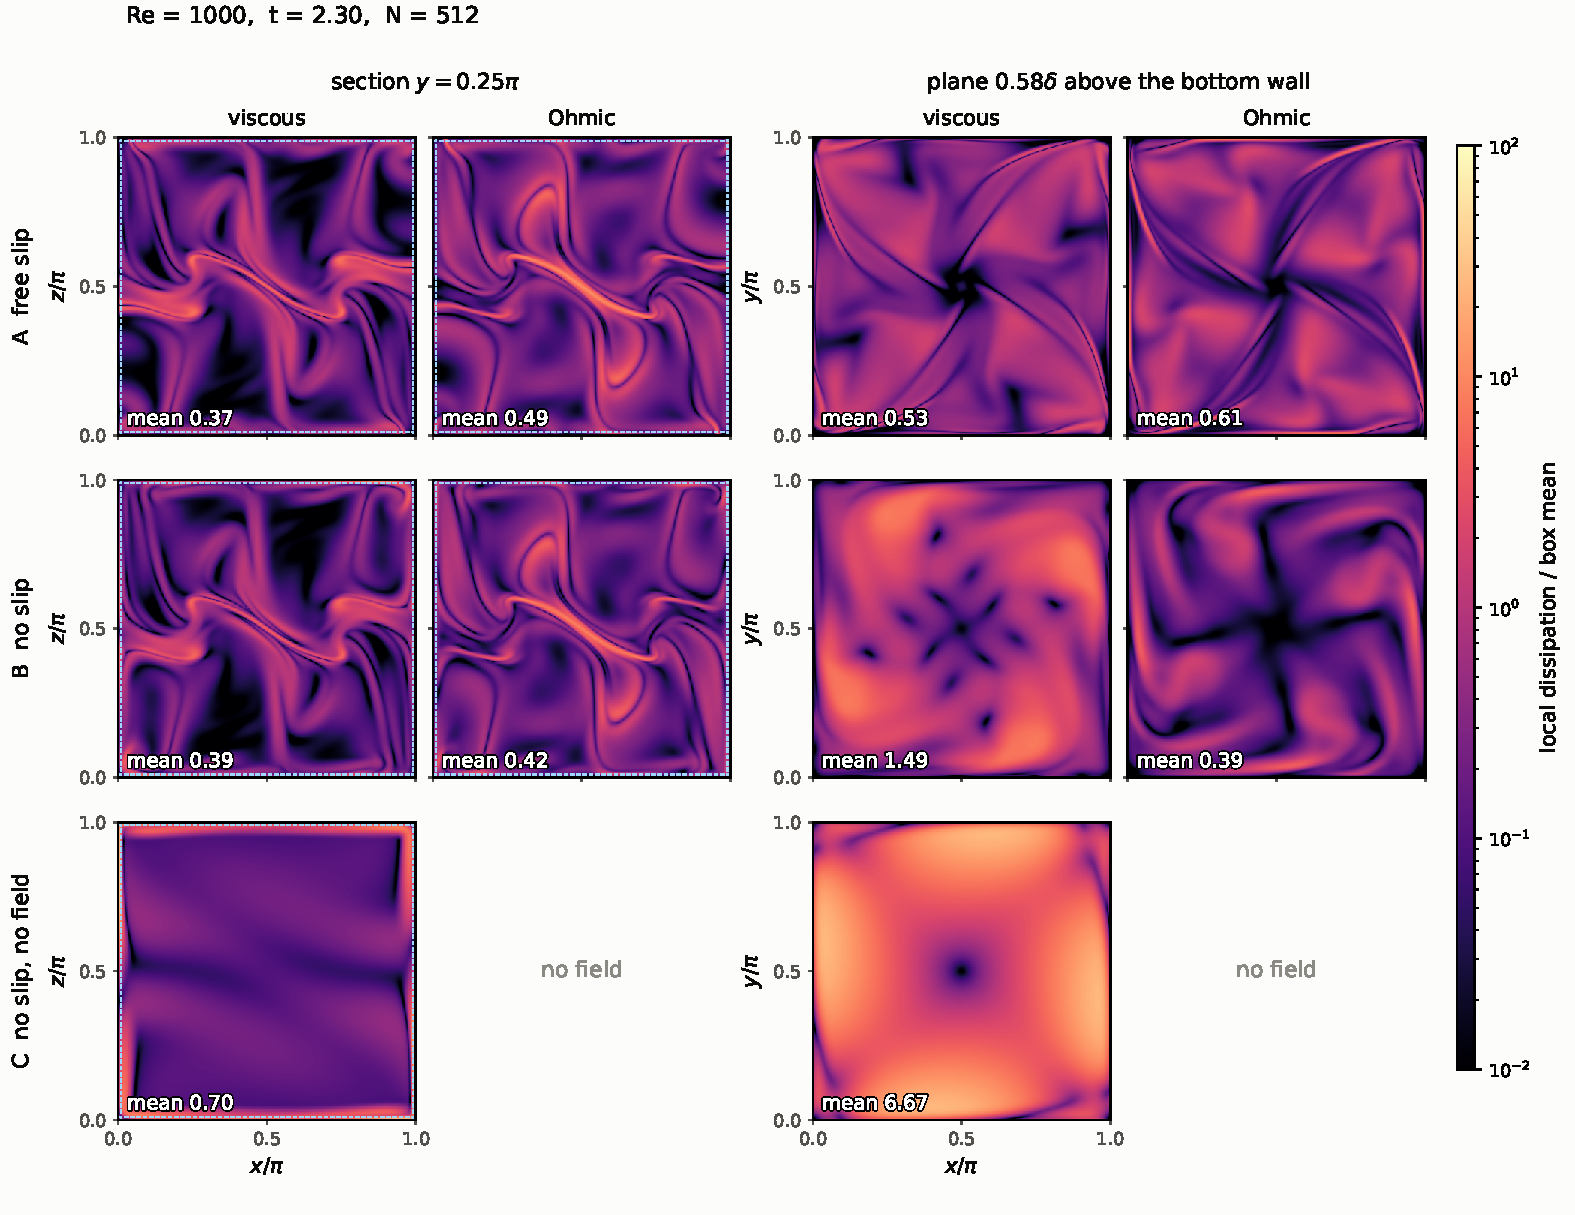
\includegraphics[width=\textwidth]{tg_mhd_snap_t2.3.pdf}
\caption{\label{fig:snap23}Where the dissipation sits, at $\Rey=1000$ and $t=2.3$
(B's turbulent peak), on the finer grid ($N=512$). Rows: the free-slip box A, the
no-slip box B and the box without a field C. Columns: the viscous and Ohmic
dissipation, $\nu|\bm\omega|^2$ and $\eta|\bm{j}|^2$, in the vertical section
$y=\pi/4$, with dashed lines at $\delta$ from its four walls, and in the plane
$0.58\delta$ above the bottom wall. One logarithmic colour scale, relative to each
box's mean dissipation at that time; each panel gives its plane's mean.}
\end{figure*}

\begin{figure*}
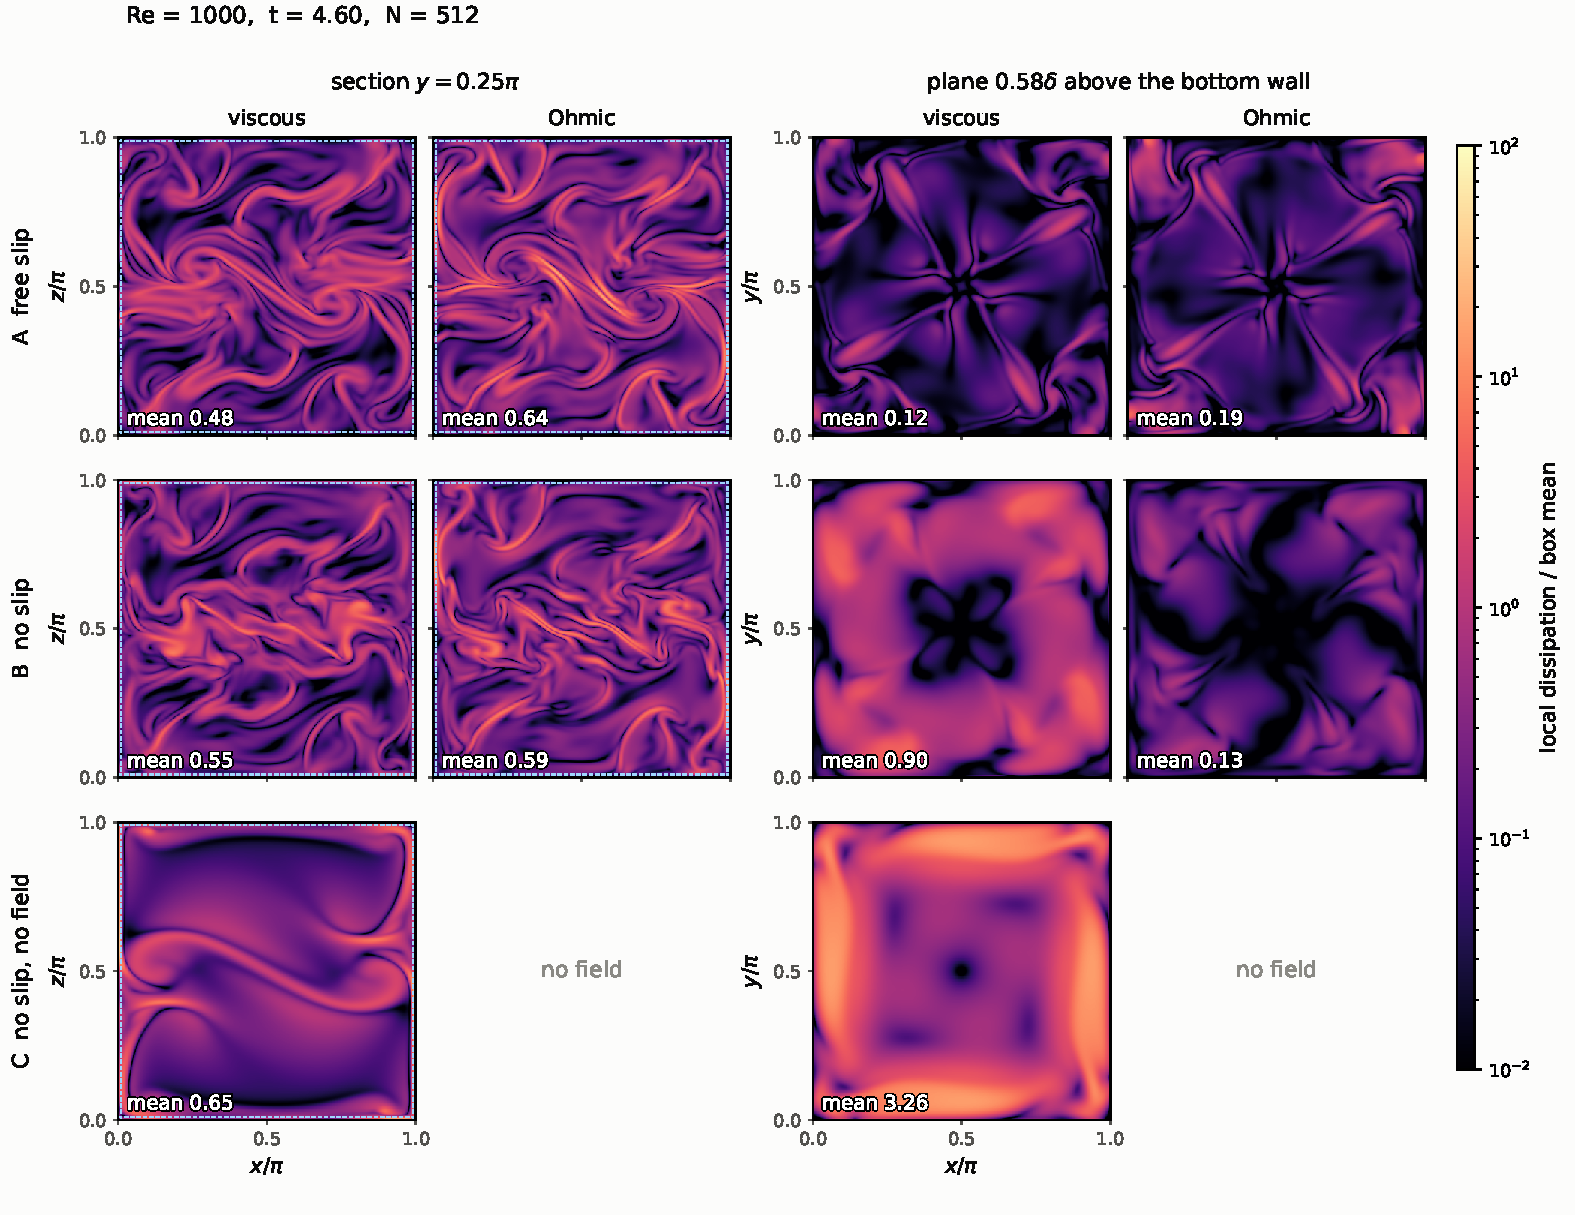
\includegraphics[width=\textwidth]{tg_mhd_snap_t4.6.pdf}
\caption{\label{fig:snap46}As Fig.~\ref{fig:snap23}, at $t=4.6$, by the later
maxima of the dissipation.}
\end{figure*}

\begin{figure*}
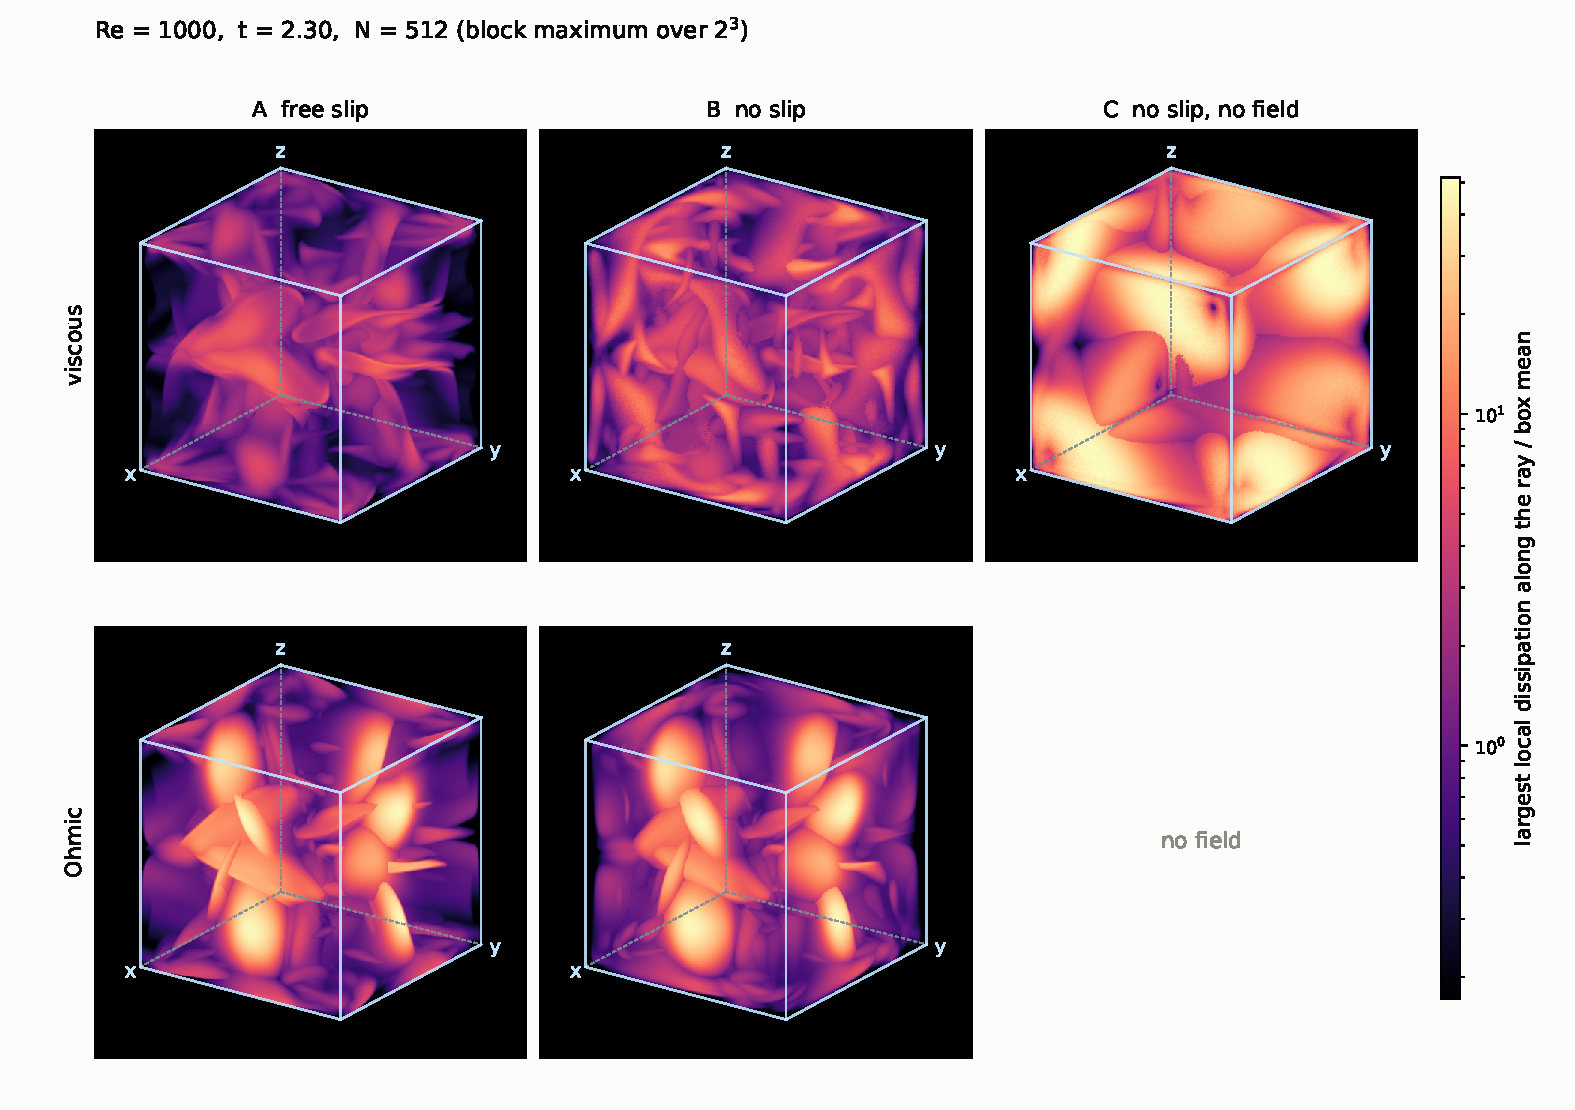
\includegraphics[width=\textwidth]{tg_mhd_3d_t2.3.pdf}
\caption{\label{fig:vol23}Three-dimensional views of the local dissipation at
$\Rey=1000$ and $t=2.3$, on the finer grid. Columns: the boxes A, B and C; rows: the
viscous and Ohmic dissipation. Each pixel is the largest value along an oblique line
of sight (maximum-intensity projection) through the volume, reduced to $256^3$ by the
maximum over $2^3$ blocks, relative to the box mean. The far half is dimmed as a
depth cue, which must not be read as an intensity; hidden edges of the box are
dashed. One logarithmic colour scale, shared with Fig.~\ref{fig:vol46}.}
\end{figure*}

\begin{figure*}
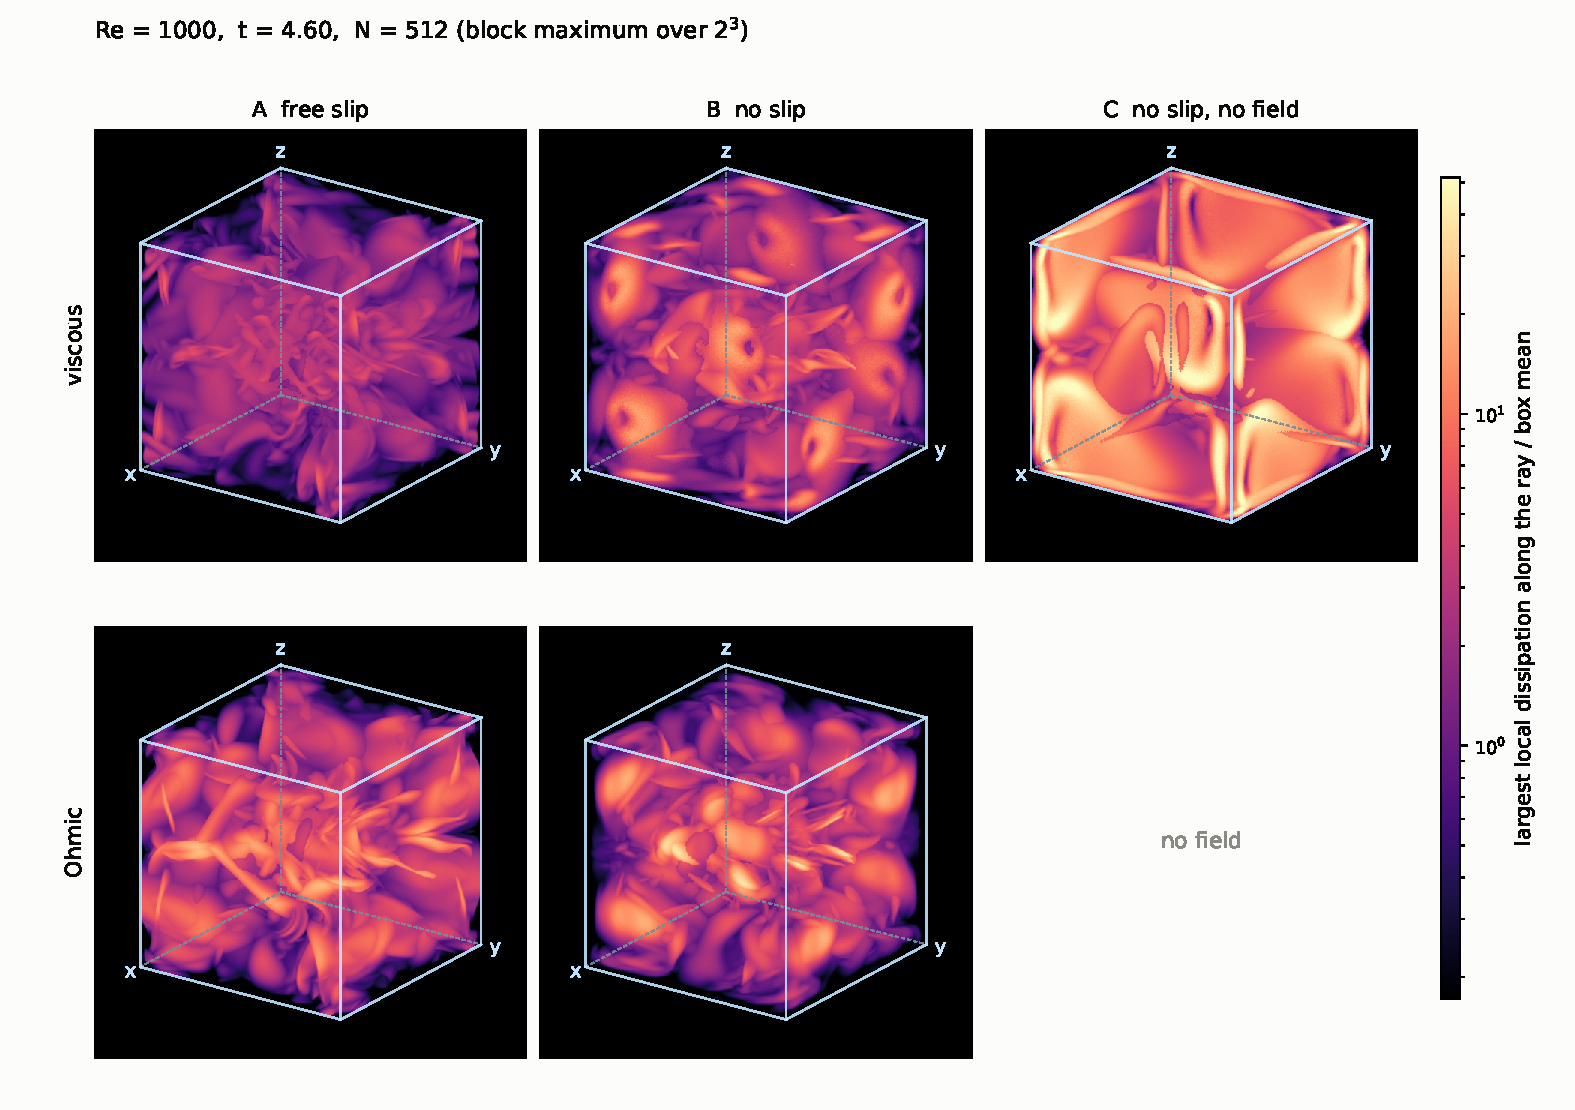
\includegraphics[width=\textwidth]{tg_mhd_3d_t4.6.pdf}
\caption{\label{fig:vol46}As Fig.~\ref{fig:vol23}, at $t=4.6$, on the same colour
scale.}
\end{figure*}

\subsection{Insulating walls}

The pair A$'$, B$'$ was meant to show whether the result needs a conducting wall. It
cannot. A$'$ passes the gate (worst $0.8$\%), and $88$\% of the dissipation within
$\delta$ of its walls is Ohmic ($F_1=0.31$ and $0.27$ at $\Rey=500$ and $1000$). B$'$
has no turbulent peak by $t=10$ at either $\Rey$. So B$'-$A$'$ ($+0.32$ and $+0.42$
over $t=2$--$10$) compares a box that has not become turbulent with one that has, and
under a different initial field from B$-$A. We draw no conclusion from it.

%===============================================================================
\section{Discussion}
\label{sec:discussion}
%===============================================================================

\emph{What the data settle.} Every measure we tried agrees on four statements. First,
a no-slip wall takes more of the dissipation next to it than a free-slip one. B$-$A is
positive and far outside its band at every $\Rey$: at the peak, at every probe from
$t=1.5$ to $10$ (where it is at least $0.019$), and over every time and energy window. Second, the excess is viscous,
and the near-wall Ohmic dissipation is lower, not higher, than at a free-slip
conducting wall, by 40--45\% in absolute terms. Third, the no-slip wall layer
intensifies with $\Rey$: B's wall dissipation density rises monotonically in every
window, while A's stays near $0.4$ of the mean. Fourth, at the one rung where the
hydrodynamic box is turbulent, the field moves dissipation away from the walls: the
box without a field dissipates $33$\% of its energy within $\delta$ of the walls, the
box with one $9.9$\%.

\emph{What they do not settle.} The question that motivated the work was whether the
wall share holds as $\Rey$ grows, and it has a registered answer: ``cascade''. That
answer rests on the peak switching from B's early maximum to its later one. A reading
that does not depend on one instant depends instead on a window. B$-$A is flat over
the window around the peaks and falls by 18--43\% over windows that reach
further into the decay, and aligning the windows on each run's energy moves the
ambiguity rather than removing it. Over a factor of eight in $\Rey$, the trend of a
decaying flow's wall share cannot be separated from the dependence of that share on
the phase of the decay. We therefore claim neither outcome. The cascade verdict stands
as the result of the test we registered, and we record that equally reasonable
readings would not have produced it.

The layer we measure has the Prandtl thickness $\delta\propto\Rey^{-1/2}$, not Kato's
$\propto\Rey^{-1}$.\cite{kato1984} Over $t=2$--$10$, B's share within $\delta$ falls
as $\Rey^{-0.19}$ and A's as $\Rey^{-0.29}$, both more slowly than the volume of the
layer, which falls as $\Rey^{-1/2}$. Whether a finite part of the dissipation remains
at the walls as $\Rey\to\infty$ cannot be decided from these data.

\emph{A conjecture for the Ohmic deficit.} At a free-slip conducting wall the
tangential flow reaches the wall, and with $\BB\cdot\bm{n}=0$ and
$\partial_n\BB_t=0$ it can stretch tangential field along it, building current sheets
next to the wall. In A the near-wall dissipation is mostly Ohmic, and the snapshots
of Sec.~\ref{sec:fields} show current sheets crossing the plane $0.58\delta$ above
the wall. A no-slip wall stops the tangential flow, and with it the induction in the
layer: in B that plane carries $0.68$--$0.79$ of A's Ohmic dissipation and several
times its viscous dissipation. The snapshots are consistent with the conjecture but do
not test its mechanism, which needs the induction term itself in the layer, and they
show one class of walls at two instants.

\emph{What the protocol bought.} Had the decision rule not been fixed in advance, any
window of Table~\ref{tab:windows} could have been chosen after seeing the data. Over
$t=2$--$6$ it would have supported ``walls hold'', over $t=5$--$10$ ``cascade''. Fixing
the rule did not make the observable robust, and it was not. But it made the
fragility something to report rather than something to choose
around.\cite{gelman2014} In a decaying flow a quantity read ``at the peak'' compares
runs at different times whenever the dissipation has more than one maximum of similar
height, and TG flows, with their sequences of sheet formation and
collision,\cite{lee2008,pouquet2010} are such flows. Before reading a trend from one
instant of a transient, the time series at every parameter value should be inspected,
and more than one definition of ``when'' should be tried.

\emph{Limitations.} One initial condition, of high symmetry, in one realization; unit
magnetic Prandtl number; and $\Rey\le2000$, set by the memory of one GPU, since
resolving $\delta$ with about $4.5$ spacings makes $N$ grow as $\Rey^{1/2}$. The method
is weakly compressible. The Mach control bounds its effect at $\Rey\le1000$, but it was
not repeated at $\Rey=2000$, where the lattice Mach number is largest ($0.133$). The
regularized edges and corners do not conserve mass exactly, though the drift stays
below $4.4\times10^{-5}$. A forced, statistically stationary box would remove the
ambiguity of ``when'' altogether, since the share would become a time average with a
standard error. It is the natural next experiment, with its own decision rule fixed
before it runs.

%===============================================================================
\section{Conclusions}
%===============================================================================

We isolated what no-slip walls do to decaying MHD turbulence by solving the
Taylor--Green MHD flow in its closed fundamental box with free-slip and no-slip walls
and nothing else changed, and we fixed the observable and the decision rule before the
runs. No-slip walls add dissipation in a layer $\Rey^{-1/2}$ thick at every Reynolds
number from $250$ to $2000$. The excess is viscous and comes with less Ohmic
dissipation at the wall, and the wall layer intensifies as $\Rey$ grows. Snapshots
of the local dissipation show the same contrast in space: current sheets cross the
near-wall layer of the free-slip box, and a broad viscous layer, with weaker currents,
lines the no-slip walls. The pre-registered reading, the excess at the dissipation peak, falls between $\Rey=1000$
and $2000$, which is the outcome we had called ``cascade''. It does so because the
peak switches from one maximum of the dissipation to another. Over this range of
$\Rey$ the trend of the wall share depends on when it is measured, and its sign does
not.

\begin{acknowledgments}
The computations used the Computational Shared Facility (CSF3) of The University of
Manchester.
% TODO(author): funding.
% TODO(author): AIP Publishing asks for any use of AI tools to be disclosed here or
% in the methods; decide the wording.
\end{acknowledgments}

\section*{Author declarations}
\subsection*{Conflict of interest}
The author has no conflicts to disclose.

\section*{Data availability}
The code (both implementations), the job scripts with the decision rules fixed before
the runs, the time series and wall-distance profiles of every run, the plane means of
the field snapshots, the analysis tools, and the script that produces every number in
this paper are in the M3LB repository, \url{https://github.com/alexderosis/M3LB}. The
field dumps behind Figs.~\ref{fig:snap23}--\ref{fig:vol46} (11\,GB per run) are
available from the author.
% TODO(author): confirm the repository is public, and cite a tagged release or DOI.

\bibliography{refs}

\end{document}
